\section{TE wave}
Question: Draw the plot showing dependence of $r_E$ and $\phi_E$ upon incidence angle for TE wave. Explain the origin and the meaning of characteristic points on this plot. Indicate orientation of the $E$ and $H$ vectors with respect to incidence plane.\bigskip

%% https://sci-hub.do/https://www.osapublishing.org/josaa/viewmedia.cfm?uri=josaa-21-8-1559&seq=0

\nocite{optics}

Light can be modelled as the electromagnetic disturbances -- a wave -- propagating through the electromagnetic field. In optocommunication we use a plane wave solution to the Maxwell's equations, which describes the changes of electric $\vec{E}$ and magnetic $\vec {B}$ fields, presented in Figure~\ref{fig:plane-wave}. We call such a wave a transverse electric and magnetic field (TEM) wave. 
\begin{figure}[h]
    \centering
    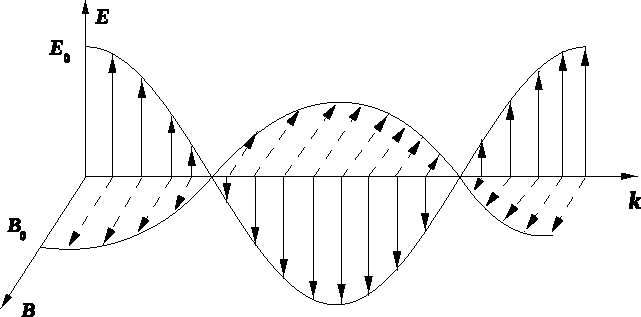
\includegraphics[width=0.7\textwidth]{images/TM_wave_plane_wave.pdf}
    \caption{A homogeneous plane wave; electric and magnetic fields are transverse to the direction of propagation and also to each other. From~\cite{optics}}
    \label{fig:plane-wave}
\end{figure}

We may also distinguish the TE and TH modes -- in the TE mode $\vec{E}$ changes are orthogonal to the incidence plane. In a three-dimensional Cartesian coordinate system with basis $B = \{\bm{\hat{n}}, \bm{\hat{\pi}}, \bm{\hat{\sigma}}\}$ and propagation direction $\bm{k}$ as presented in Figure~\ref{fig:boundary}, electric field variations would be observed only in $\bm{\sigma}$ axis, thus:
\begin{align*}
    \vec{E} &= [0, E_y, 0] & \vec{H} &= [H_x, 0, H_z]
\end{align*}
\begin{figure}[ht]
    \centering
    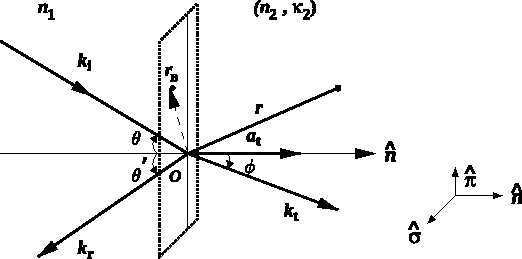
\includegraphics{images/reflection_at_boundary.pdf}
    \caption{Reflection and transmission of a wave at a plane boundary. From~\cite{optics}}
    \label{fig:boundary}
\end{figure}
Based on~\cite[ch.~1.7]{optics} and~\cite{Urbanczyk} we may denote a reflection coefficient for the orthogonally polarized wave $r_\sigma$  as
\begin{equation}
    r_{\sigma ext} = \frac{n_1\cos{\theta} - n_2\cos{\phi}}{n_1\cos{\theta} + n_2\cos{\phi}},
\end{equation}
where the refraction angle $\phi$ is
\begin{equation}
    \phi = \arcsin{\frac{n_1\sin{\theta}}{n_2}}
\end{equation}
for the external reflections (when $\theta < \theta_c$) and
\begin{equation}
    \label{eq:r-sig-int}
    r_{\sigma int} = \frac{n_1\cos{\theta} - i\sqrt{n_1^2\sin^2{\theta} - n_2^2}}{n_1\cos{\theta} + i\sqrt{n_1^2\sin^2{\theta} - n_2^2}} = e^{-i2\phi_0},
\end{equation}
where the phase change $2\phi_0$ is
\begin{equation}
    \phi_0 = \arctan{\frac{\sqrt{n_1^2\sin^2{\theta} - n_2^2}}{n_1\cos{\theta}}}.
\end{equation}
for the internal reflections (when $\theta > \theta_c$). 

As we may see in Equation~\ref{eq:r-sig-int} the reflection coefficient has unit magnitude for any angle exceeding the critical angle, thus the reflection is total.  $r_{\sigma int}$ being complex implies that the reflected field will not be in phase with the incident one and its phase change will grow from $2\phi_0=0$ at $\theta = \theta_c$ to $2\phi_0=\pi$ at $\theta = \frac{\pi}{2}$.

\begin{figure}[h]
    \centering
    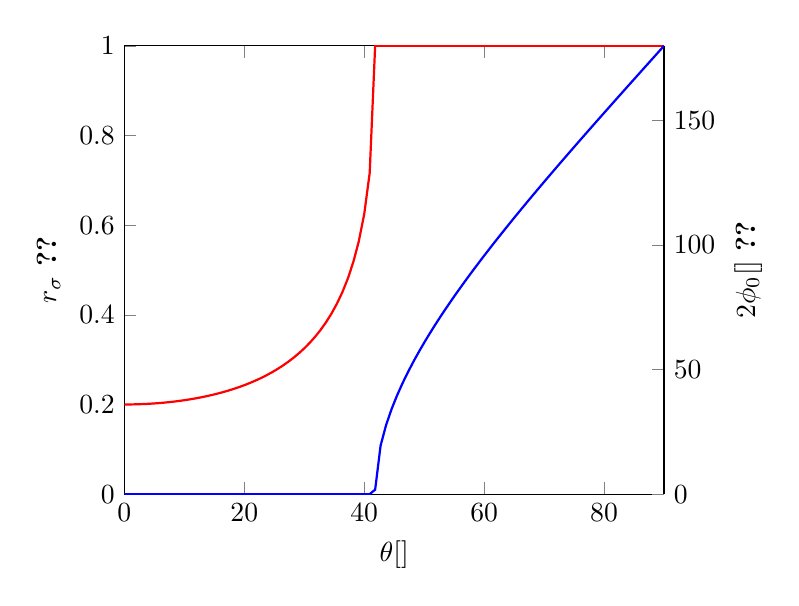
\begin{tikzpicture}
        \begin{axis}[
            axis y line* = left,
            xmin = 0, xmax= 90,
            ymin = 0, ymax = 1,
            xlabel = {$\theta [\si{\degree}]$},
            ylabel = {$r_\sigma$ \ref{plot:r}},
        ]
        \addplot[
            color=red,
            thick,
        ] table[row sep=crcr] {
            0	0.2\\
            0.909090909090909	0.200075548358143\\
            1.81818181818182	0.200302474323788\\
            2.72727272727273	0.200681623239942\\
            3.63636363636364	0.20121441295981\\
            4.54545454545455	0.20190284744675\\
            5.45454545454545	0.202749536175467\\
            6.36363636363636	0.20375771970972\\
            7.27272727272727	0.204931301959892\\
            8.18181818181818	0.206274889768904\\
            9.09090909090909	0.207793840642697\\
            10	0.20949431963852\\
            10.9090909090909	0.211383366659131\\
            11.8181818181818	0.21346897568415\\
            12.7272727272727	0.215760187815008\\
            13.6363636363636	0.218267200434693\\
            14.5454545454545	0.221001495310923\\
            15.4545454545455	0.223975989131789\\
            16.3636363636364	0.227205210796962\\
            17.2727272727273	0.230705510849594\\
            18.1818181818182	0.234495309798338\\
            19.0909090909091	0.238595393847125\\
            20	0.243029268863856\\
            20.9090909090909	0.247823586476549\\
            21.8181818181818	0.253008660269373\\
            22.7272727272727	0.25861909556895\\
            23.6363636363636	0.264694563859932\\
            24.5454545454545	0.271280763335456\\
            25.4545454545455	0.27843062181496\\
            26.3636363636364	0.286205819319164\\
            27.2727272727273	0.294678738238488\\
            28.1818181818182	0.303934994516478\\
            29.0909090909091	0.31407677226833\\
            30	0.325227291513248\\
            30.9090909090909	0.337536910103694\\
            31.8181818181818	0.351191643599362\\
            32.7272727272727	0.366425370146303\\
            33.6363636363636	0.383537849309218\\
            34.5454545454545	0.402922298925275\\
            35.4545454545455	0.425109485950506\\
            36.3636363636364	0.450842156114725\\
            37.2727272727273	0.481209720776053\\
            38.1818181818182	0.517915584981499\\
            39.0909090909091	0.563881382374634\\
            40	0.624914480999515\\
            40.9090909090909	0.716331282587392\\
            41.8181818181818	1\\
            42.7272727272727	1\\
            43.6363636363636	1\\
            44.5454545454545	1\\
            45.4545454545455	1\\
            46.3636363636364	1\\
            47.2727272727273	1\\
            48.1818181818182	1\\
            49.0909090909091	1\\
            50	1\\
            50.9090909090909	1\\
            51.8181818181818	1\\
            52.7272727272727	1\\
            53.6363636363636	1\\
            54.5454545454545	1\\
            55.4545454545455	1\\
            56.3636363636364	1\\
            57.2727272727273	1\\
            58.1818181818182	1\\
            59.0909090909091	1\\
            60	1\\
            60.9090909090909	1\\
            61.8181818181818	1\\
            62.7272727272727	1\\
            63.6363636363636	1\\
            64.5454545454545	1\\
            65.4545454545455	1\\
            66.3636363636364	1\\
            67.2727272727273	1\\
            68.1818181818182	1\\
            69.0909090909091	1\\
            70	1\\
            70.9090909090909	1\\
            71.8181818181818	1\\
            72.7272727272727	1\\
            73.6363636363636	1\\
            74.5454545454545	1\\
            75.4545454545455	1\\
            76.3636363636364	1\\
            77.2727272727273	1\\
            78.1818181818182	1\\
            79.0909090909091	1\\
            80	1\\
            80.9090909090909	1\\
            81.8181818181818	1\\
            82.7272727272727	1\\
            83.6363636363636	1\\
            84.5454545454545	1\\
            85.4545454545455	1\\
            86.3636363636364	1\\
            87.2727272727273	1\\
            88.1818181818182	1\\
            89.0909090909091	1\\
            90	1\\
            };\label{plot:r}
        \end{axis}
        \begin{axis}[
            axis y line* = right,
            axis x line = none,
            xmin = 0, xmax= 90,
            ymin = 0, ymax = 180,
            ylabel = {$2\phi_0[\si{\degree}]$ \ref{plot:phi}},
        ]
        \addplot[
            color=blue,
            thick,
        ] table[row sep=crcr] {
0	0\\
0.909090909090909	0\\
1.81818181818182	0\\
2.72727272727273	0\\
3.63636363636364	0\\
4.54545454545455	0\\
5.45454545454545	0\\
6.36363636363636	0\\
7.27272727272727	0\\
8.18181818181818	0\\
9.09090909090909	0\\
10	0\\
10.9090909090909	0\\
11.8181818181818	0\\
12.7272727272727	0\\
13.6363636363636	0\\
14.5454545454545	0\\
15.4545454545455	0\\
16.3636363636364	0\\
17.2727272727273	0\\
18.1818181818182	0\\
19.0909090909091	0\\
20	0\\
20.9090909090909	0\\
21.8181818181818	0\\
22.7272727272727	0\\
23.6363636363636	0\\
24.5454545454545	0\\
25.4545454545455	0\\
26.3636363636364	0\\
27.2727272727273	0\\
28.1818181818182	0\\
29.0909090909091	0\\
30	0\\
30.9090909090909	0\\
31.8181818181818	0\\
32.7272727272727	0\\
33.6363636363636	0\\
34.5454545454545	0\\
35.4545454545455	0\\
36.3636363636364	0\\
37.2727272727273	0\\
38.1818181818182	0\\
39.0909090909091	0\\
40	0\\
40.9090909090909	0\\
41.8181818181818	1.79598353355014\\
42.7272727272727	19.4985527790721\\
43.6363636363636	27.6686978780157\\
44.5454545454545	34.0490313573982\\
45.4545454545455	39.5165098076433\\
46.3636363636364	44.4098364890434\\
47.2727272727273	48.9019135841755\\
48.1818181818182	53.0949117606083\\
49.0909090909091	57.0550291633055\\
50	60.827982315635\\
50.9090909090909	64.4468620944837\\
51.8181818181818	67.9365018645714\\
52.7272727272727	71.3160805468255\\
53.6363636363636	74.6007602857732\\
54.5454545454545	77.8027627548109\\
55.4545454545455	80.9321024404152\\
56.3636363636364	83.9971015358059\\
57.2727272727273	87.0047608978192\\
58.1818181818182	89.9610332914974\\
59.0909090909091	92.871028584335\\
60	95.7391704772668\\
60.9090909090909	98.5693180354601\\
61.8181818181818	101.364861201285\\
62.7272727272727	104.128796773537\\
63.6363636363636	106.86378951345\\
64.5454545454545	109.572221781262\\
65.4545454545455	112.25623422553\\
66.3636363636364	114.917759418943\\
67.2727272727273	117.55854987984\\
68.1818181818182	120.180201585379\\
69.0909090909091	122.784173834979\\
70	125.371806137018\\
70.9090909090909	127.944332650903\\
71.8181818181818	130.502894608788\\
72.7272727272727	133.048551057815\\
73.6363636363636	135.582288198766\\
74.5454545454545	138.105027545984\\
75.4545454545455	140.617633092989\\
76.3636363636364	143.120917636091\\
77.2727272727273	145.615648382451\\
78.1818181818182	148.102551948301\\
79.0909090909091	150.582318836149\\
80	153.055607466088\\
80.9090909090909	155.523047825116\\
81.8181818181818	157.985244789165\\
82.7272727272727	160.442781164964\\
83.6363636363636	162.896220492662\\
84.5454545454545	165.346109644938\\
85.4545454545455	167.792981254162\\
86.3636363636364	170.237355995653\\
87.2727272727273	172.679744752279\\
88.1818181818182	175.120650683363\\
89.0909090909091	177.560571219063\\
90	180\\
        };\label{plot:phi}
        \end{axis}
    \end{tikzpicture}
    \caption{Variation of reflection coefficient $r_E$ and phase change $2\phi_0$ for $\frac{n_1}{n_2}=1.5$ computed in \MATLAB}
\end{figure}
